% 第 9 章 变分公式
% 来源：KneserPaper, sec-general.tex 小节 "The first-order term as a derivative on the
% parabolic stratum"（Lemma gen-banach, Prop. gen-linear, Thm gen-variation,
% Cor. gen-variation, Remarks gen-cocycle, gen-variation）；docs/kappa-variation-zh.md。
% 本章不新增宏。

\chapter{变分公式}\label{ch:variation}

第~\ref{ch:first-order} 章把一阶系数 $\kappa^{(n)}$ 写成了抛物轨道上的一个绝对收敛级数（\cref{thm:first-order}）。
级数给出了数值，却没有说明这个数「是什么」。本章回答这个问题。

答案是几何的。把所有靠近 $g$ 的映射放在一个 Banach 空间里。有二重不动点的映射构成一个复解析超曲面 $\Pstr$，
称为\textbf{抛物层}（parabolic stratum）。在实映射中，它把「有两个实不动点」的映射与「有一对复共轭不动点」的映射分开。
不变量 $\tau_n$ 定义在前一侧；在 $\Pstr$ 上，对应的量是 $B_n\ee^{2\pi\ii na}$。
我们证明：这两个量拼成的函数在 $g$ 处沿任何开折方向都有单侧导数，并且这个导数是一个连续线性泛函。
$\kappa^{(n)}$ 就是它沿开折方向 $X$ 的导数，按 $X=X(0)\cdot1+(X-X(0))$ 分成法向和切向两部分：
\[
 \kappa^{(n)}=\ktr^{(n)}(g)+\frac{\Dfun_n(g)\bigl[X-X(0)\bigr]}{4a_2X(0)} .
\]
切向部分是 horn 映射沿 $\Pstr$ 的导数，是抛物芽的形变理论里的对象；法向部分是芽 $g$ 的一个数 $\ktr^{(n)}(g)$。

这个分解立刻回答了「$\kappa^{(n)}$ 有没有闭式」的问题：同一个芽配不同的开折方向，$\operatorname{Re}\kappa^{(n)}$ 可以从 $-0.0102$ 变到 $395$，
所以 $\kappa^{(n)}$ 不是芽的函数。它还说明 tetration 为什么是「标准」例子：底数方向与平移方向只差一个无穷小共轭。

\begin{goals}
\item 同调算子 $\Lop\phi=\phi\circ g-g'\phi$ 描述无穷小共轭；它的形式余核是 $\operatorname{span}\{1,u^3\}$。
\item 抛物层 $\Pstr$ 是复解析超曲面，$T_g\Pstr=\{Y:Y(0)=0\}$；常数方向 $1$ 是法向。
\item 一致模型对 Banach 参数全纯，由此得到连续线性泛函 $\Lfun_n$，它同时给出开折的一阶项和 $\Pstr$ 上的导数。
\item 变分公式（\cref{thm:variation}）：$\kappa^{(n)}$ = 法向常数 $\ktr^{(n)}(g)$ + horn 不变量的切向导数。
\item $\operatorname{Re}\kappa^{(n)}$ 只依赖开折方向模 $\Lop$ 的类；$\ktr^{(n)}$ 在坐标变换下按上闭链变化，不是芽的不变量。
\item horn 变分由正则化的轨道级数（Melnikov 型公式）计算；数值上公式两边吻合到 $10^{-17}$（$n=1$）。
\end{goals}

%====================================================================
\section{问题：一阶系数依赖什么}\label{ch9:sec:question}

回忆第~\ref{ch:unfolding} 章的设定（\cref{def:unfolding}）。$g(u)=u+a_2u^2+a_3u^3+\cdots$ 是实抛物芽，$a_2>0$；
开折 $f_s$ 满足
\begin{equation}\label{ch9:eq:direction}
 f_s=g-sX+O(s^2),\qquad \gamma=X(0)>0 .
\end{equation}
我们称 $X$ 为开折的\textbf{方向}（direction）。由 \cref{prop:scales}，$p=-\log\lambda_1\log\lambda_2=4a_2\gamma s+O(s^2)$。
第~\ref{ch:first-order} 章证明了：若 $B_n\ne0$，则
\begin{equation}\label{ch9:eq:kappa-recall}
 \log\frac{\tau_n}{B_n\ee^{2\pi\ii na}}=\kappa^{(n)}p+O(p^{10/9}),\qquad
 \kappa^{(n)}=\frac{\delta t_n}{4a_2\gamma B_n}-\frac{2\pi\ii n\,\delta t_0}{4a_2\gamma},
\end{equation}
其中 $\delta t_m$ 是闸门线上函数 $\delta T$ 的 Fourier 系数，$\delta T$ 由正则化的轨道级数给出（\cref{thm:first-order}；全阶版本见 \cref{thm:all-orders}）。

\begin{lemma}\label{ch9:lem:first-jet}
$\kappa^{(n)}$ 只依赖于芽 $g$、方向 $X$ 和基点 $\ustar$，与 $f_s$ 的 $O(s^2)$ 项无关。
\end{lemma}

\begin{proof}
在 \cref{thm:first-order} 的公式里，参数只通过三处进入：一致模型时间 $\Psi_s$ 对 $s$ 的导数、一步误差 $F_s$ 对 $s$ 的导数、
以及轨道导数 $\dot u_k=\partial_sf_s^k(u)|_{s=0}$。由链式法则，前两者只依赖 $\partial_sf_s|_{s=0}=-X$，
而 $\dot u_k$ 满足递推 $\dot u_{k+1}=g'(u_k)\dot u_k-X(u_k)$，$\dot u_0=0$，也只依赖 $X$。
最后 $p'(0)=4a_2\gamma$ 只依赖 $X(0)$。
\end{proof}

所以我们可以写 $\kappa^{(n)}=\kappa^{(n)}[g;X]$。它是 $X$ 的什么样的函数？\cref{ch9:tab:preview} 给出了第一个线索。

\begin{table}[htbp]
\centering\small
\caption{同一个芽 $g=\ee^u-1$、不同方向 $X$ 的一阶系数（$n=1$，基点 $\ustar=1/\ee-1$）。
数据来自 \texttt{docs/kappa\_variation.py}，45 位运算，输出文件 \texttt{docs/data/kappa-variation-exp.txt}。}
\label{ch9:tab:preview}
\begin{tabular}{lll}
\toprule
方向 $X$ & $\operatorname{Re}\kappa^{(1)}$ & $\operatorname{Im}\kappa^{(1)}$\\
\midrule
$1$ & $-0.0101990063458974$ & $19.1021373259046$\\
$(1+u)\ee^u$（tetration） & $-0.0101990063458974$ & $-0.0132509561825067$\\
$1+0.6u^2$ & $39.5149228923293$ & $62.4195598999261$\\
$1+0.3u+0.5u^4$ & $395.094296950776$ & $-224.037840614510$\\
\bottomrule
\end{tabular}
\end{table}

表中有两个现象。第一，$\operatorname{Re}\kappa^{(1)}$ 随方向剧烈变化，因此 $\kappa^{(n)}$ 不可能只是 $g$（或 $B_n$、$a$、$\rho$）的函数。
第二，平移方向 $X=1$ 与 tetration 的方向 $X=(1+u)\ee^u$ 给出相同的实部，虚部却不同。
本章的目标是解释这两个现象：实部只依赖于 $X$ 模无穷小共轭的类（\cref{ch9:sec:homological}），
而对这个类的依赖是仿射的，斜率是 horn 不变量沿抛物层的导数（\cref{ch9:sec:formula}）。

%====================================================================
\section{同调算子与无穷小共轭}\label{ch9:sec:homological}

\subsection{定义}
固定 $r>0$ 足够小，使 $g$ 在 $D_{2r}=\{|u|<2r\}$ 上全纯且 $g(\overline{D_r})\subset D_{2r}$。
记 $\Ocal_r$ 为 $D_r$ 上有界全纯函数构成的 Banach 空间，范数为上确界范数。

\begin{definition}\label{ch9:def:Lop}
芽 $g$ 的\textbf{同调算子}（homological operator）是
\[
 \Lop:\Ocal_{2r}\to\Ocal_r,\qquad \Lop\phi=\phi\circ g-g'\,\phi .
\]
它是有界线性算子。若 $\phi$ 在实轴上取实值，就称 $\phi$ 是实的。
\end{definition}

这个算子的意义是下面的计算。

\begin{lemma}[无穷小共轭]\label{ch9:lem:infinitesimal-conjugacy}
设 $\phi\in\Ocal_{2r}$，$\psi_t=\id+t\phi$。则对 $|t|$ 足够小，在 $D_{r/2}$ 上
\[
 \psi_t^{-1}\circ g\circ\psi_t=g-t\,\Lop\phi+O(t^2) .
\]
更一般地，若 $f_s=g-sX+O(s^2)$，则 $\psi_s^{-1}\circ f_s\circ\psi_s=g-s(X+\Lop\phi)+O(s^2)$。
这里的 $O(\cdot)$ 是在 $\Ocal_{r/2}$ 的范数下。
\end{lemma}

\begin{proof}
$g\circ\psi_t(u)=g(u+t\phi(u))=g(u)+t\,g'(u)\phi(u)+O(t^2)$。
又 $\psi_t^{-1}(v)=v-t\phi(v)+O(t^2)$（由 $\psi_t(\psi_t^{-1}v)=v$ 比较一阶项）。代入 $v=g\circ\psi_t(u)=g(u)+O(t)$ 得
\[
 \psi_t^{-1}\circ g\circ\psi_t=g+t\,g'\phi-t\,\phi\circ g+O(t^2)=g-t\Lop\phi+O(t^2).
\]
所有余项都由 Cauchy 估计在 $D_{r/2}$ 上一致控制。第二个公式同理：$f_s$ 的 $-sX$ 项在共轭下只产生 $-sX+O(s^2)$。
\end{proof}

于是，把方向 $X$ 换成 $X+\Lop\phi$（$\phi$ 实）相当于在一阶上对开折作实解析共轭 $\psi_s=\id+s\phi$。结合 \cref{ch9:lem:first-jet} 与 \cref{cor:invariance}，这已经提示 $\operatorname{Re}\kappa^{(n)}$ 在这个替换下不变；\cref{cor:variation} 将在本章的局部设定下直接证明这一点。
注意 $\Lop\phi(0)=\phi(0)-g'(0)\phi(0)=0$，所以这个替换不改变横截性 $\gamma=X(0)$。

\subsection{形式余核}
在形式幂级数环 $\C[[u]]$ 上同样定义 $\Lop\phi=\phi\circ g-g'\phi$。

\begin{proposition}\label{ch9:prop:formal-coker}
\begin{enumerate}
\item 对每个 $k\ge0$，
\[
 \Lop(u^k)=(k-2)a_2\,u^{k+1}+\Bigl((k-3)a_3+\tbinom k2a_2^2\Bigr)u^{k+2}+O(u^{k+3}) .
\]
\item $\C[[u]]=\C\cdot1\ \oplus\ \C\cdot u^3\ \oplus\ \Lop(\C[[u]])$（直和）。
\item $\ker\Lop$ 是一维的，由一个首项为 $u^2$ 的级数张成。
\end{enumerate}
\end{proposition}

\begin{proof}
(1) 由二项式展开，
$g(u)^k=u^k(1+a_2u+a_3u^2+\cdots)^k=u^k+ka_2u^{k+1}+\bigl(ka_3+\binom k2a_2^2\bigr)u^{k+2}+\cdots$，
而 $g'(u)u^k=u^k+2a_2u^{k+1}+3a_3u^{k+2}+\cdots$。相减即得。

(2) 记 $[Y]_j$ 为 $Y$ 中 $u^j$ 的系数。由 (1)，$\Lop(u^k)$ 从 $u^{k+1}$ 开始，首项系数 $(k-2)a_2$ 仅在 $k=2$ 时为零。

\emph{生成.} 给定 $Y\in\C[[u]]$，我们逐阶构造 $\phi=\sum\phi_ku^k$。因为 $\Lop\phi$ 没有常数项，必须取 $c_0=[Y]_0$。
比较 $u^1,u^2$ 的系数，依次解出 $\phi_0=-[Y]_1/(2a_2)$ 与 $\phi_1$（首项系数 $-a_2\ne0$）。
$u^3$ 的系数中 $\phi_2$ 的贡献为零（因 $(2-2)a_2=0$），而 $\phi_k$（$k\ge3$）不贡献，
所以令 $c_3=[Y]_3-[\Lop(\phi_0+\phi_1u)]_3$，并取 $\phi_2=0$。
对 $j\ge4$，$u^j$ 的系数方程是 $(j-3)a_2\phi_{j-1}+(\text{已定的量})=[Y]_j$，可唯一解出 $\phi_{j-1}$。
于是 $Y=c_0+c_3u^3+\Lop\phi$。

\emph{直和.} 设 $c_0+c_3u^3=\Lop\phi$。常数项给出 $c_0=0$；$u^1,u^2$ 的系数依次给出 $\phi_0=\phi_1=0$；
这时 $[\Lop\phi]_3=0$，故 $c_3=0$。

(3) 若 $\Lop\phi=0$，上一段的论证给出 $\phi_0=\phi_1=0$，而 $\phi_2$ 任意；$\phi_2$ 确定之后，$u^j$（$j\ge4$）的方程唯一确定 $\phi_{j-1}$。
所以 $\ker\Lop$ 由 $\phi_2=1$ 的唯一解张成。
\end{proof}

\begin{remark}[余核的解释]\label{ch9:rem:coker-meaning}
两个余核方向各有含义。方向 $1$ 是开折参数本身：$g-s$ 把二重不动点分裂开。
方向 $u^3$ 对应迭代留数 $\rho=1-a_3/a_2^2$ 的变化：对 $Y=y_2u^2+y_3u^3+\cdots$，沿 $g-tY$ 有
\[
 \frac{\dd\rho}{\dd t}\Big|_{t=0}=\frac{a_2y_3-2a_3y_2}{a_2^3},
\]
而 $\rho$ 是芽在保持 $0$ 的（形式）共轭下的不变量（线性换元同时缩放 $a_2$ 与 $a_3$，比值 $a_3/a_2^2$ 不变），所以它在 $\Lop\phi$（$\phi=O(u)$，此时 $\Lop\phi=O(u^2)$）上的导数为零（\cref{ch9:ex:drho}）。
这与开折的形式分类相符：鞍结开折的形式不变量是一个参数和一个留数函数\cite{ChristopherRousseau}。
$\ker\Lop$ 的生成元是 $g$ 的形式无穷小生成元（\cref{ch9:ex:kernel}）。

在解析范畴里，$\Ocal_r/\Lop(\Ocal_{2r})$ 远比 $\operatorname{span}\{1,u^3\}$ 大：芽的解析分类除形式不变量外还有 \'Ecalle--Voronin 模，
它是无穷维的\cite{Ecalle1981,Voronin1981}。启发式地说，多出来的余核方向就是模空间的切方向。
本章不需要、也不证明这一说法；下面用到的只是 $\Lop$ 的像在一个具体意义下「对实部不可见」（\cref{cor:variation}）。
\end{remark}

\begin{example}\label{ch9:ex:coboundaries}
三个具体的上边界（即 $\Lop$ 的像中的元素）。
\begin{enumerate}
\item 二次芽 $g=u+u^2$：$\Lop(u)=u+u^2-(1+2u)u=-u^2$。
\item 指数芽 $g=\ee^u-1$：$\Lop(u)=\ee^u-1-u\ee^u$。
\item 指数芽与常数加线性函数：$\Lop(-2-u)=(-2-(\ee^u-1))-\ee^u(-2-u)=(1+u)\ee^u-1$。
\end{enumerate}
第三个等式说：tetration 的方向 $X=(1+u)\ee^u$（\cref{ch9:ex:tetration-direction}）满足 $X-1\in\Lop(\Ocal_{2r})$。
\end{example}

\begin{example}\label{ch9:ex:tetration-direction}
tetration 的族 $w\mapsto b^w$ 在仿射坐标 $w=\ee(1+u)$ 下是 $f_s(u)=\ee^{-s+(1-s)u}-1$，$s=1-\ee\log b$，基点 $w_0=1$ 对应 $\ustar=1/\ee-1$。对 $s$ 求导，
$\partial_sf_s(u)|_{s=0}=-(1+u)\ee^u$，所以 $X=(1+u)\ee^u$，$\gamma=1$，$a_2=\tfrac12$，$4a_2\gamma=2=p'(0)$。
对二次族 $w^2+c$，取 $w=\tfrac12+u$、$c=\tfrac14-s$，得 $f_s(u)=u+u^2-s$，这是平移开折，$X=1$。
对 $v-\sin v+c$，取 $v=\tfrac\pi2+u$、$c=1-s$，得 $f_s(u)=u+(1-\cos u)-s$，也是平移开折。
\end{example}

%====================================================================
\section{抛物层}\label{ch9:sec:stratum}

\subsection{对称函数与判别式}
设 $f\in\Ocal_r$ 靠近 $g$。因为 $g(u)-u=a_2u^2(1+O(u))$ 在圆周 $|u|=r/2$ 上不为零（$r$ 小），由 Rouché 定理，
当 $\|f-g\|$ 足够小时，$f-\id$ 在 $D_{r/2}$ 内恰有两个零点（计重数），记为 $u_1[f],u_2[f]$。

\begin{lemma}\label{ch9:lem:symmetric}
存在 $g$ 在 $\Ocal_r$ 中的邻域 $U$，使下面的量都是 $f\in U$ 的全纯函数：
\[
 e_1[f]=u_1+u_2,\qquad e_2[f]=u_1u_2,\qquad D[f]=e_1^2-4e_2=(u_1-u_2)^2,
\]
以及 Weierstrass 分解 $f(u)-u=q[f](u)\,\mathsf k[f](u)$ 中的二次多项式 $q[f](u)=u^2-e_1u+e_2$ 和余因子 $\mathsf k[f]\in\Ocal_{r/2}$，
$\mathsf k[f]$ 在 $D_{r/2}$ 上无零点，$\mathsf k[g](0)=a_2$。并且 $e_2[f]=f(0)/\mathsf k[f](0)$。
\end{lemma}

\begin{proof}
由辐角原理，对 $j=1,2$，
\[
 u_1^j+u_2^j=\frac1{2\pi\ii}\oint_{|u|=r/2}u^j\,\frac{f'(u)-1}{f(u)-u}\,\dd u .
\]
被积函数在圆周上关于 $f$ 全纯（$f\mapsto f'(u)$ 是有界线性映射，$f(u)-u$ 在圆周上远离零），所以幂和关于 $f$ 全纯，
$e_1=u_1+u_2$，$e_2=\tfrac12\bigl(e_1^2-(u_1^2+u_2^2)\bigr)$ 也是。
余因子 $\mathsf k[f]=(f-\id)/q[f]$ 在 $D_{r/2}$ 内全纯（零点相消），并由 Cauchy 积分
$\mathsf k[f](u)=\frac1{2\pi\ii}\oint_{|\zeta|=r/2}\frac{f(\zeta)-\zeta}{q[f](\zeta)(\zeta-u)}\,\dd\zeta$（$|u|<r/2$）关于 $f$ 全纯。
在 $u=0$ 处 $f(0)=q[f](0)\mathsf k[f](0)=e_2\mathsf k[f](0)$。$\mathsf k[g](u)=(g(u)-u)/u^2$，故 $\mathsf k[g](0)=a_2$。
这是 Weierstrass 预备定理（\cref{thm:weierstrass-prep}）带 Banach 参数的形式，这里的积分公式直接给出了参数全纯性。
\end{proof}

这里「全纯」是 Banach 空间意义下的：映射在每点 Fr\'echet 复可微。本章反复使用下面的经典事实\cite[§§5--8]{Mujica1986}：
一个局部有界的映射，若在每条复直线上全纯（G-全纯），则全纯；全纯映射的复合、Cauchy 积分、一致收敛极限仍然全纯；
全纯映射有 Cauchy 估计。另见附录~\ref{app:tools}。

\subsection{抛物层是超曲面}

\begin{definition}\label{ch9:def:stratum}
$g$ 附近的\textbf{抛物层} $\Pstr$ 是 $U$ 中在 $D_{r/2}$ 内有二重不动点的映射的集合，即 $\Pstr=\{f\in U:D[f]=0\}$。
$Y\in\Ocal_r$ 称为 $\Pstr$ 在 $g$ 处的\textbf{切向量}，指存在 $\Pstr$ 中的曲线 $g-tY+O(t^2)$。
\end{definition}

注意切向量的符号约定：切向量 $Y$ 对应的曲线是 $g-tY$，与开折 $f_s=g-sX$ 的约定一致。

\begin{proposition}\label{ch9:prop:submersion}
\begin{enumerate}
\item $D$ 在 $g$ 处是淹没：$\dd D[g](H)=-4H(0)/a_2$，其中 $\dd D[g](H)$ 表示沿曲线 $g+tH$ 的导数。
\item $\Pstr$ 在 $g$ 附近是 $\Ocal_r$ 中的复解析超曲面，切空间为
\[
 T_g\Pstr=\{Y\in\Ocal_r:\ Y(0)=0\} .
\]
\item 每个 $Y\in T_g\Pstr$ 都是 $\Pstr$ 中一条全纯曲线 $t\mapsto g-tY+c(t)\cdot1$ 的切向量，其中 $c$ 全纯，$c(t)=O(t^2)$。
若 $Y$ 是实的，这条曲线由实映射组成。
\end{enumerate}
\end{proposition}

\begin{proof}
(1) 因 $e_1[g]=0$，$\dd(e_1^2)[g]=2e_1[g]\,\dd e_1[g]=0$。由 \cref{ch9:lem:symmetric}，
$e_2[g+tH]=(g+tH)(0)/\mathsf k[g+tH](0)=tH(0)/\mathsf k[g+tH](0)$，所以 $\dd e_2[g](H)=H(0)/a_2$。于是 $\dd D[g](H)=-4H(0)/a_2$。
这个线性泛函不为零（取 $H=1$）。

(2) $\ker\dd D[g]=\{H:H(0)=0\}$ 有闭补空间 $\C\cdot1$。由 Banach 空间上的隐函数定理，
存在 $\ker\dd D[g]$ 中 $0$ 的邻域上的全纯函数 $c$，$c(0)=0$，$\dd c(0)=0$，使在 $g$ 附近
$D[g+H+c\cdot1]=0$（$H\in\ker\dd D[g]$）当且仅当 $c=c(H)$。所以 $\Pstr$ 局部是图像 $\{g+H+c(H)\cdot1\}$，切空间是 $\ker\dd D[g]$。

(3) 取 $H=-tY$，曲线 $t\mapsto g-tY+c(-tY)\cdot1$ 在 $\Pstr$ 中。因 $\dd c(0)=0$，$c(-tY)=O(t^2)$。
若 $Y$ 实，记 $f^\star(u)=\overline{f(\bar u)}$。$D[f^\star]=\overline{D[f]}$，所以 $c(H^\star)=\overline{c(H)}$，由唯一性，实 $H$ 给出实 $c(H)$。
\end{proof}

\begin{remark}[实的图景]\label{ch9:rem:real-picture}
对实的 $f\in U$，$D[f]$ 是实数。$D>0$ 时两个不动点 $u_1<u_2$ 是实的；由 $f(u)-u=q\mathsf k$ 和 $\mathsf k>0$，
$f'(u_1)=1+(u_1-u_2)\mathsf k(u_1)<1<f'(u_2)$，所以左边的不动点自动是吸引的。$D<0$ 时两个不动点复共轭。
对开折 \eqref{ch9:eq:direction}，$D[f_s]=4\gamma s/a_2+O(s^2)$，这正是 \cref{prop:scales} 证明中出现的判别式。
所以 $\gamma>0$ 等价于：开折曲线在 $g$ 处横截 $\Pstr$，并进入 $D>0$ 的一侧。
\end{remark}

\begin{figure}[htbp]
\centering
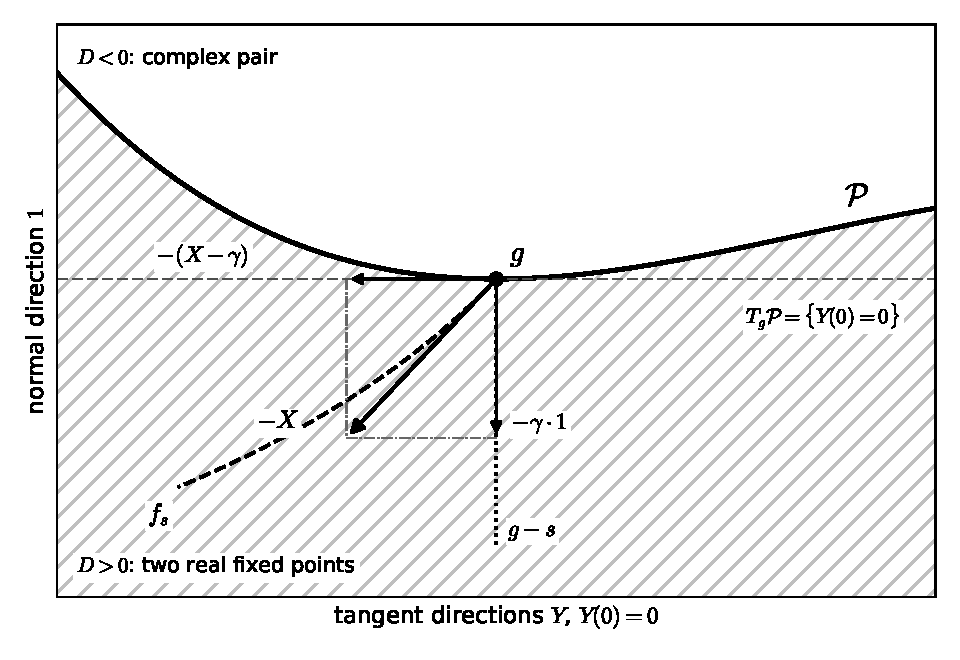
\includegraphics[width=0.78\textwidth]{figures/fig9_stratum.pdf}
\caption{$g$ 附近映射空间的示意图。横轴代表切方向 $T_g\Pstr=\{Y(0)=0\}$，纵轴代表常数方向 $1$。
粗实线是抛物层 $\Pstr$；阴影区 $D>0$ 是有两个实不动点的实映射，上方 $D<0$ 是有一对复共轭不动点的映射。
虚线是开折 $f_s=g-sX+O(s^2)$，其速度 $-X$ 分解为法向分量 $-\gamma\cdot1$ 与切向分量 $-(X-\gamma)$。
点线是平移开折 $g-s$。（脚本 \texttt{figures/fig9\_stratum.py}）}
\label{ch9:fig:stratum}
\end{figure}

\cref{ch9:fig:stratum} 是本章的几何图景。不变量 $\tau_n$ 定义在阴影区；我们要说明它与 $\Pstr$ 上的 $B_n\ee^{2\pi\ii na}$
拼成一个在 $g$ 处「一阶光滑」的函数，然后对这个函数的导数作切向、法向分解。

%====================================================================
\section{一致模型的 Banach 全纯性}\label{ch9:sec:banach}

本节把第~\ref{ch:first-order} 章的一致模型（\cref{lem:uniform-model}）从单参数族推广到 Banach 参数。
回忆它的构造。对 $f$ 靠近 $g$，令 $u_1,u_2$ 为 $f$ 在 $D_{r/2}$ 内的不动点，$q=q[f]$，$\mathsf k=\mathsf k[f]$，
\[
 A[f](x,y)=\frac1{\log\bigl(1+(x-y)\mathsf k[f](x)\bigr)},\qquad A_1=A[f](u_1,u_2),\quad A_2=A[f](u_2,u_1),
\]
所以 $D[f]\ne0$ 时 $A_j=1/\log f'(u_j)$。取整数 $N\ge1$，一致模型时间与一步误差为
\begin{align*}
 \Psi[f](u)&=A_1\log(u-u_1)+A_2\log(u-u_2)+P[f](u),\\
 F[f](u)&=\Psi[f](f(u))-\Psi[f](u)-1,
\end{align*}
其中 $P[f]=\sum_{i=1}^{2N-2}\mathsf p_i[f]u^i$ 是使 $F[f]$ 被 $q[f]^N$ 整除的多项式；对数分支按 \cref{lem:uniform-model}(1) 的约定，
即 $|u|>\delta$ 时 $\log(u-u_j)=\log u+\Log(1-u_j/u)$。记 $\nu[f]=A_1+A_2$。

\begin{lemma}\label{ch9:lem:banach}
固定 $N\ge3$。缩小 $r$ 之后，在 $g$ 于 $\Ocal_r$ 中的某个邻域上：
\begin{enumerate}
\item $\nu[f]$ 和一步误差 $F[f]=q[f]^N\Gamma[f]$ 关于 $f$ 全纯，后者取值于 $D_{r/2}$ 上有界全纯函数的空间；
\item 对每个 $\delta\in(0,r/2)$，在一个（更小的）邻域上，模型时间 $\Psi[f]-\nu[f]\log u$ 关于 $f$ 全纯，取值于圆环 $\delta<|u|<r/2$ 上有界全纯函数的空间；
\item 对反射逆映射 $G[f](v)=-f^{-1}(-v)$ 同样成立。
\end{enumerate}
\end{lemma}

\begin{proof}
\cref{lem:uniform-model} 的证明由三步组成，我们逐步检查它们对 Banach 参数的全纯依赖。

\emph{第一步：预备与除法。} $e_1,e_2,q[f],\mathsf k[f]$ 关于 $f$ 全纯（\cref{ch9:lem:symmetric}）。
Weierstrass 除法 $\chi=q[f]\cdot(\text{商})+(\text{余式})$ 由 Cauchy 积分给出，商和余式都关于 $(f,\chi)$ 全纯。

\emph{第二步：对角线上的可去性。} 令 $\chi(x)$ 是 $(f,x,y,u)$ 的全纯函数。考虑
\[
 \Theta=A[f](x,y)\,\chi(y)+A[f](y,x)\,\chi(x),\qquad \Theta'=A[f](x,y)\,\chi(x)+A[f](y,x)\,\chi(y).
\]
由 $1/\log(1+z)=1/z+\tfrac12+O(z)$，$A[f](x,y)=\frac1{(x-y)\mathsf k[f](x)}+\tfrac12+(x-y)\mathsf q[f](x,y)$，$\mathsf q$ 全纯。
所以 $\Theta$ 的奇异部分是 $\bigl[\chi(y)/\mathsf k(x)-\chi(x)/\mathsf k(y)\bigr]/(x-y)$，分子在对角线 $x=y$ 上为零；
$\Theta'$ 的奇异部分 $\bigl[\chi(x)/\mathsf k(x)-\chi(y)/\mathsf k(y)\bigr]/(x-y)$ 同样可去。
因此 $\Theta,\Theta'$ 是 $(f,x,y,u)$ 的全纯函数，且关于 $x,y$ 对称。对称的全纯函数是初等对称函数 $(x+y,xy)$ 的全纯函数
（对每个固定的其他变量，这是关于两个变量的对称收敛幂级数的经典事实；参数依赖由 Cauchy 积分表示保持）。
代入 $(x+y,xy)=(e_1[f],e_2[f])$，得到 $f$ 的全纯函数。应用于
\begin{itemize}
\item $\chi\equiv1$ 于 $\Theta'$：得到 $\nu[f]$；
\item $\chi(x)=\Log(1-x/u)$ 于 $\Theta'$（$|u|>\delta$，$|u_j|<\delta/2$）：得到 $\Psi[f]-\nu[f]\log u-P[f]$；
\item $\chi(x)=\log\bigl(1+(u-x)\mathsf k[f](u)\bigr)$ 于 $\Theta$：得到 $F^{\log}[f]=A_1\log\frac{f-u_1}{u-u_1}+A_2\log\frac{f-u_2}{u-u_2}-1$，
  因为 $(f(u)-u_1)/(u-u_1)=1+(u-u_2)\mathsf k(u)$。
\end{itemize}

\emph{第三步：线性方程组.} $D[f]\ne0$ 时 $F^{\log}[f](u_j)=A_j\log f'(u_j)-1=0$，所以 $F^{\log}[f]$ 被 $q[f]$ 除的余式在两个不同点为零，
是零。余式关于 $f$ 全纯，而 $\{D\ne0\}$ 在 $U$ 中稠密，所以余式恒为零：$F^{\log}[f]=q[f]\varphi[f]$，$\varphi$ 全纯。
同理 $u\mapsto f(u)^i-u^i=q[f]\,d_i[f]$。把 $\varphi+\sum_i\mathsf p_id_i$ 除以 $q[f]^{N-1}$，余式的 $2N-2$ 个系数关于 $f$ 全纯、关于 $\mathsf p=(\mathsf p_i)$ 仿射，
矩阵记为 $M[f]$。在 $f=g$ 处余式就是模 $u^{2N-2}$ 的 Taylor 多项式，$d_i[g]=ia_2u^{i-1}+O(u^i)$，所以 $M[g]$ 是下三角的，
对角元 $ia_2\ne0$。于是在 $g$ 附近 $\mathsf p[f]=-M[f]^{-1}\operatorname{rem}(\varphi[f])$ 关于 $f$ 全纯，且 $F[f]=q[f]^N\Gamma[f]$，$\Gamma[f]$ 全纯。

每一步都把全纯映射复合、作 Cauchy 积分或求逆，所以结论成立。对 $G[f]$，先用 Banach 空间上的反函数定理得到 $f\mapsto f^{-1}$ 在 $D_{r/2}$ 附近全纯，
再重复上面的论证。
\end{proof}

\begin{remark}
\cref{ch9:lem:banach} 是本章唯一的技术性输入。它说的是：第~\ref{ch:first-order} 章里所有对 $s$ 的全纯依赖，
其实是对整个映射 $f$ 的全纯依赖，$s$ 只是通过 $f_s$ 进入。由此，任何「对 $s$ 求导」都可以改写成「沿方向 $-X$ 的方向导数」。
\end{remark}

%====================================================================
\section{线性泛函 \texorpdfstring{$\Lfun_n$}{L\_n}}\label{ch9:sec:linear}

\subsection{设定}
本章所说的\textbf{开折}，指实解析曲线 $s\mapsto f_s\in\Ocal_r$，$f_0=g$，满足 \eqref{ch9:eq:direction} 与 $\gamma>0$。
不需要 \cref{def:unfolding} 中 (H1) 那样的整体假设：我们用的 $\tau_n$ 是闸门线上局部转移 $\mathcal A\circ(\mathcal S^\sharp)^{-1}$ 的不变量
$t_n\ee^{-2\pi\ii nt_0}$，而这正是 \cref{thm:reduction}、\cref{thm:confluence} 与第~\ref{ch:first-order} 章的证明所使用的全部内容。
基点取为实数 $\ustar\in(-r/2,0)$，满足 $g$ 在 $[\ustar,0]$ 上递增且 $g(u)>u$（$u\in[\ustar,0)$）；
对 $f$ 靠近 $g$，同样的性质在吸引不动点左侧成立。对整函数族（满足 (H1)），基点可以像第~\ref{ch:first-order} 章那样用 $f^m$ 搬运到远处，论证不变。

记 $\ell=[0,1]+\ii Y_*$ 为闸门线（\cref{thm:confluence}），$v(z)=\Phirep[g]^{-1}(z)$。对 $f$ 靠近 $g$，令
\[
 \mathcal A[f](u)=\Psi[f](u)+\sum_{k\ge0}F[f](f^ku)
\]
（在吸引花瓣中；在其余的基本域上用 $\mathcal A[f]\circ f^m-m$ 延拓），$\mathcal S[f]$ 为反射族 $G[f]$ 的同样构造给出的排斥时间。

\begin{definition}\label{ch9:def:invariant}
对实的 $f$ 靠近 $g$、有两个实不动点（$D[f]>0$），令 $\Ifun_n[f]=\tau_n[f]$；对 $f\in\Pstr$，令
\[
 \Ifun_n[f]=B_n[f]\,\ee^{2\pi\ii na[f]},
\]
其中 $B_n[f]$、$a[f]=\Phiatt[f](\ustar)$ 由 $f$ 在其二重不动点处的芽计算（\cref{def:horn}，用该芽的形式 Abel 函数归一化），基点仍是 $\ustar$。
\end{definition}

两种情形下，$\Ifun_n[f]$ 都是闸门线上转移 $T=\mathcal A[f]\circ\mathcal S^\sharp[f]^{-1}$ 的不变量 $t_n\ee^{-2\pi\ii nt_0}$，
其中 $\mathcal A[f]$ 按 $\mathcal A[f](\ustar)=0$ 归一化（\cref{thm:reduction} 与第~\ref{ch:first-order} 章）。

\begin{remark}[归一化的重要性]\label{ch9:rem:normalization}
这个归一化不是装饰。吸引一侧加一个常数 $c$，$T$ 变成 $T+c$，$t_0\mapsto t_0+c$，于是 $t_n\ee^{-2\pi\ii nt_0}$ 乘上 $\ee^{-2\pi\ii nc}$；
排斥一侧加常数 $c$，$T(z)$ 变成 $T(z-c)$，$t_n\mapsto t_n\ee^{-2\pi\ii nc}$，$t_0\mapsto t_0-c$，$t_n\ee^{-2\pi\ii nt_0}$ 不变。
所以只有吸引一侧需要钉住，钉在基点上。这也是 $a$ 出现在极限 $B_n\ee^{2\pi\ii na}$ 中的原因（参见 \cref{prop:base-point}）。
\end{remark}

由 \cref{thm:confluence}，$\Ifun_n$ 在 $g$ 处从 $D>0$ 的一侧连续：$\Ifun_n[f_s]\to\Ifun_n[g]$。

\subsection{泛函的定义}
在第~\ref{ch:first-order} 章 \cref{thm:first-order} 的 $\dot\tau_n$ 公式里，把每个对 $s$ 的导数换成沿 $-X$ 的方向导数：
对 $u$ 在花瓣的紧子集 $K$ 中，令
\begin{equation}\label{ch9:eq:Adot}
 \dot{\mathcal A}[X](u)=\dd\Psi[g](-X)(u)+\sum_{k\ge0}\Bigl[\dd F[g](-X)(u_k)+F[g]'(u_k)\,\dot u_k\Bigr],
\end{equation}
其中 $u_k=g^k(u)$，$\dot u_{k+1}=g'(u_k)\dot u_k-X(u_k)$，$\dot u_0=0$。在基点和花瓣以外的基本域上，用 $\dot{\mathcal A}=\dot{\mathcal A}\circ g^m+\mathcal A[g]'\circ g^m\cdot\dot u_m$ 延拓。
排斥一侧由 $G$ 同样定义 $\dot{\mathcal S}^\sharp[X]$，其中 $\mathcal S^\sharp$ 在闸门中一个固定参考点 $u_\sharp$ 处的值 $\Phirep[g](u_\sharp)$ 保持不变（第~\ref{ch:first-order} 章的归一化）。令
\begin{gather*}
 \delta T[X](z)=\dot{\mathcal A}[X](v(z))-\dot{\mathcal A}[X](\ustar)-\tilde T_0'(z)\,\dot{\mathcal S}^\sharp[X](v(z)),\\
 \tilde T_0=\horn^{-1}-a,\qquad
 \delta t_m[X]=\int_\ell\delta T[X](z)\,\ee^{-2\pi\ii mz}\,\dd z .
\end{gather*}

\begin{definition}\label{ch9:def:Lfun}
对 $X\in\Ocal_r$，定义
\[
 \Lfun_n(X)=\ee^{-2\pi\ii nt_0}\bigl(\delta t_n[X]-2\pi\ii n\,t_n\,\delta t_0[X]\bigr)
 =\ee^{2\pi\ii na}\bigl(\delta t_n[X]-2\pi\ii n\,B_n\,\delta t_0[X]\bigr),
\]
其中 $t_n=B_n$、$t_0=-a$ 是 $\tilde T_0$ 的 Fourier 系数。
\end{definition}

\begin{proposition}\label{ch9:prop:linear}
$\Lfun_n$ 是 $\Ocal_r$ 上的连续复线性泛函，并且：
\begin{enumerate}
\item 对每个方向为 $X$ 的开折，当 $s\to0^+$ 时 $\Ifun_n[f_s]=\Ifun_n[g]+s\,\Lfun_n(X)+O(s^{10/9})$；
\item 对 $\Pstr$ 中每条全纯曲线 $t\mapsto g_t$，$g_0=g$，函数 $t\mapsto\Ifun_n[g_t]$ 在 $0$ 附近全纯，且在 $0$ 处的导数是 $\Lfun_n(-\partial_tg_t|_{t=0})$。
\end{enumerate}
\end{proposition}

\begin{proof}
\emph{线性与连续性.} 由 \cref{ch9:lem:banach}，$\dd\Psi[g]$ 与 $\dd F[g]$ 是有界线性算子，$\dot u_k$ 关于 $X$ 线性，
所以 \eqref{ch9:eq:Adot} 的每一项关于 $X$ 线性。第~\ref{ch:first-order} 章的导数估计（$|\dot u_k|\le C(k+1)$，
$|\partial F|\le M'|v|^{2N-2}$，$|F'|\le M'|v|^{2N-1}$）的证明只用到 Cauchy 估计，在这里以 $\|X\|$ 为因子成立。
所以级数的项是 $O(\|X\|(R+k/2)^{2-2N})$，一致绝对收敛，$|\Lfun_n(X)|\le C\|X\|$。

(1) 对单个开折，由链式法则 $\partial_s\Psi[f_s]|_{s=0}=\dd\Psi[g](-X)$，$\partial_sF[f_s]|_{s=0}=\dd F[g](-X)$。
所以 \eqref{ch9:eq:Adot} 就是第~\ref{ch:first-order} 章的导数 $\dot{\mathcal A}$，而 $\Lfun_n(X)$ 就是 \cref{thm:first-order} 中的 $\dot\tau_n$。
\cref{thm:first-order} 给出 $\tau_n=\Ifun_n[g]+s\dot\tau_n+O(s^{10/9})$，即 (1)。

(2) 设 $g_t\in\Pstr$ 是全纯曲线，二重不动点为 $u_0(t)$。$g_t$ 在 $u_0(t)$ 处的芽的二阶系数 $a_2(t)\to a_2$。
第~\ref{ch:first-order} 章「有限轨道」引理在未扰动情形（参数为零）的证明，在坐标 $-1/(a_2(t)(u-u_0(t)))$ 中逐字成立，
给出对所有 $k$、关于小复数 $t$ 一致的花瓣估计。所以级数 $\mathcal A[g_t](u)=\Psi[g_t](u)+\sum_kF[g_t](g_t^ku)$ 一致收敛；
每一项关于 $t$ 全纯（\cref{ch9:lem:banach} 与复合）。由 Weierstrass 定理，和关于 $t$ 全纯，且 $t$ 导数可以逐项计算，
也就是把 \eqref{ch9:eq:Adot} 中的 $-X$ 换成 $\partial_tg_t|_{t=0}$ 得到的级数。

和 $s=0$ 时一样（第~\ref{ch:first-order} 章），$\mathcal A[g_t]$ 等于 $\Phiatt[g_t]$ 加一个常数：两者都满足 $g_t$ 的 Abel 方程，
而 $\Psi[g_t]$ 与 $g_t$ 的形式 Abel 函数只差一个常数和 $O((u-u_0(t))^{2N-1})$，所以 $\mathcal A[g_t]-\Phiatt[g_t]$ 沿轨道趋于常数，
由 Fatou 坐标的唯一性（\cref{thm:fatou-coordinates}）它就是常数。归一化 $\mathcal A[g_t](\ustar)=0$ 消去这个常数：
\[
 \mathcal A[g_t]-\mathcal A[g_t](\ustar)=\Phiatt[g_t]-a[g_t] .
\]
排斥一侧对 $G$ 作同样的论证；那里的加法常数不影响 $\Ifun_n$（\cref{ch9:rem:normalization}）。
闸门线上的求逆（Rouché）和 Fourier 积分关于 $t$ 全纯，所以 $\Ifun_n[g_t]$ 关于 $t$ 全纯，导数为 $\Lfun_n(-\partial_tg_t|_{t=0})$。
\end{proof}

\begin{remark}
(1) 与 (2) 的地位不同。(1) 是单侧的：$\tau_n$ 只在 $D>0$ 一侧有定义，$O(s^{10/9})$ 的余项来自第~\ref{ch:first-order} 章的头尾平衡论证。
(2) 是双侧的、全纯的：在 $\Pstr$ 上不动点不分裂，花瓣估计对复参数一致，不需要一致模型的精细结构。
两者由同一个泛函 $\Lfun_n$ 联系起来，这是 \cref{thm:variation} 的全部内容。
\end{remark}

%====================================================================
\section{变分公式}\label{ch9:sec:formula}

\begin{theorem}[变分公式]\label{thm:variation}
设 $B_n\ne0$。令
\[
 \ktr^{(n)}(g)=\frac{\Lfun_n(1)}{4a_2\,\Ifun_n[g]},\qquad
 \Dfun_n(g)[Y]=\frac{\dd}{\dd t}\Big|_{t=0}\log\Ifun_n[g_t]\quad(Y\in T_g\Pstr),
\]
其中 $g_t\in\Pstr$ 是任一满足 $g_0=g$、$\partial_tg_t|_{t=0}=-Y$ 的全纯曲线。由 \cref{ch9:prop:linear}(2)，
$\Dfun_n(g)[Y]=\Lfun_n(Y)/\Ifun_n[g]$，所以 $\Dfun_n(g)$ 是良定的线性泛函。则对 $g$ 的每个方向为 $X$ 的开折，
\[
 \kappa^{(n)}=\ktr^{(n)}(g)+\frac{\Dfun_n(g)\bigl[X-X(0)\bigr]}{4a_2\,X(0)} .
\]
特别地，$\ktr^{(n)}(g)$ 是平移开折 $g-s$ 的一阶系数，并且
\[
 \operatorname{Re}\kappa^{(n)}=\operatorname{Re}\ktr^{(n)}(g)+\frac{\dd\log|B_n|\,\bigl[X-X(0)\bigr]}{4a_2\,X(0)},
\]
其中 $\dd\log|B_n|[Y]=\frac{\dd}{\dd t}\log|B_n[g_t]|$ 沿 $\Pstr$ 中的实曲线计算。
\end{theorem}

\begin{proof}
由 \cref{prop:scales}，$p=4a_2\gamma s+O(s^2)$，$\gamma=X(0)$。由 \cref{ch9:prop:linear}(1) 和 $B_n\ne0$（故 $\Ifun_n[g]\ne0$），
\[
 \log\frac{\Ifun_n[f_s]}{\Ifun_n[g]}=s\,\frac{\Lfun_n(X)}{\Ifun_n[g]}+O(s^{10/9})=p\,\frac{\Lfun_n(X)}{4a_2\gamma\,\Ifun_n[g]}+O(p^{10/9}),
\]
所以 $\kappa^{(n)}=\Lfun_n(X)/(4a_2\gamma\,\Ifun_n[g])$。写 $X=\gamma\cdot1+(X-\gamma)$。由 \cref{ch9:prop:submersion}，$X-\gamma\in T_g\Pstr$；
由定义，$\Lfun_n(X-\gamma)=\Ifun_n[g]\,\Dfun_n(g)[X-\gamma]$。由线性，
\[
 \kappa^{(n)}=\frac{\gamma\,\Lfun_n(1)+\Ifun_n[g]\,\Dfun_n(g)[X-\gamma]}{4a_2\gamma\,\Ifun_n[g]}
 =\ktr^{(n)}(g)+\frac{\Dfun_n(g)[X-\gamma]}{4a_2\gamma}.
\]
取 $X=1$ 即知 $\ktr^{(n)}(g)$ 是平移开折的一阶系数。

实部：设 $f\in\Pstr$ 是实的。它的二重不动点 $u_0=e_1[f]/2$ 是实的，$f(u)-u=(u-u_0)^2\mathsf k[f](u)>0$（$u\ne u_0$ 靠近 $0$），
基点在 $f$ 的实吸引轴上，所以 $a[f]$ 是实数，$|\Ifun_n[f]|=|B_n[f]|$。对实的 $X$，由 \cref{ch9:prop:submersion}(3) 取 $\Pstr$ 中切于 $X-\gamma$ 的实曲线 $g_t$。
沿这条曲线 $\operatorname{Re}\log\Ifun_n[g_t]=\log|B_n[g_t]|$，所以 $\operatorname{Re}\Dfun_n(g)[X-\gamma]=\dd\log|B_n|[X-\gamma]$。
\end{proof}

公式的几何意义见 \cref{ch9:fig:stratum}：$\log\Ifun_n$ 在 $g$ 处的「导数」$\Lfun_n/\Ifun_n[g]$ 作用在速度 $-X$ 上
（符号已吸收进约定），法向分量给出 $\gamma\cdot4a_2\ktr^{(n)}$，切向分量给出 horn 不变量沿 $\Pstr$ 的导数。

\begin{remark}[为什么不用两参数论证]\label{ch9:rem:two-parameter}
公式最初是用另一种论证猜出来的。设 $X_1=O(u^2)$，令 $g_t=g-tX_1$，考虑两参数族 $G(s,t)=g_t-s\gamma$。
对固定的 $t$，$G(\cdot,t)$ 是抛物芽 $g_t$ 的平移开折，由第~\ref{ch:first-order} 章，
\[
 \log\tau_n(s,t)=\log\Ifun_n[g_t]+\ktr^{(n)}(g_t)\,p(s,t)+O(p^{1+\beta}) .
\]
在对角线 $t=s$ 上，$G(s,s)=g-s(\gamma+X_1)$ 正是方向为 $\gamma+X_1$ 的开折；对 $s$ 求导就得到 \cref{thm:variation} 对这类方向的情形（一般方向再用下面的 \cref{ch9:lem:gauge} 去掉一次项）。
这个论证的缺口在于余项：需要 $O(p^{1+\beta})$ 关于 $t$ 一致，即重新检查第~\ref{ch:first-order} 章的所有常数对芽参数的依赖。
\cref{ch9:prop:linear} 绕开了这一点：它只在 $g$ 一个点上用到第~\ref{ch:first-order} 章的单侧估计，而在 $\Pstr$ 上只用到全纯性。
两个论证的差别是一个常见的教训：与其在一族对象上要求估计一致，不如找一个线性化的对象（这里是 $\Lfun_n$），让一致性由线性代替。
\end{remark}

\begin{remark}[另一侧]
$\Ifun_n$ 只在 $D\ge0$ 的一侧有定义。在 $D<0$ 一侧（\cref{ch9:fig:stratum} 的上方，复共轭不动点，Lavaurs 方向），
相应的对象是 Lavaurs 映射与扰动 Fatou 坐标，它们对参数全纯依赖\cite{Shishikura2000,InouShishikura}。
变分公式的类比在那一侧是否成立、法向常数能否从那一侧读出，本书不讨论。
\end{remark}

\begin{corollary}\label{cor:variation}
\begin{enumerate}
\item $\operatorname{Re}\kappa^{(n)}$ 只通过 $X$ 模无穷小共轭 $\Lop\phi$（$\phi\in\Ocal_{2r}$ 实）的类依赖于 $X$。
  数值上，它不是芽 $g$ 单独的函数（\cref{ch9:sec:numerics}）。
\item 对 tetration，方向是 $X=(1+u)\ee^u$，而 $X-1=\Lop(-2-u)$。所以 $\operatorname{Re}\kappa^{(n)}=\operatorname{Re}\ktr^{(n)}(\ee^u-1)$。
\end{enumerate}
\end{corollary}

\begin{proof}
(1) $\Lop\phi(0)=0$，所以 $X\mapsto X+\Lop\phi$ 不改变 $X(0)$，而在 $X-X(0)$ 上加了 $\Lop\phi\in T_g\Pstr$。由 \cref{thm:variation}，只需证
$\dd\log|B_n|[\Lop\phi]=0$。曲线 $g_t=(\id+t\phi)^{-1}\circ g\circ(\id+t\phi)$ 在 $\Pstr$ 中（共轭保持二重不动点），
由 \cref{ch9:lem:infinitesimal-conjugacy} 它等于 $g-t\Lop\phi+O(t^2)$，所以它的切向量是 $\Lop\phi$。对实的 $t$，
Fatou 坐标被实共轭 $\psi_t=\id+t\phi$ 搬运：$\Phiatt[g_t]-\Phiatt[g]\circ\psi_t$ 与 $\Phirep[g_t]-\Phirep[g]\circ\psi_t$ 都是常数
（两者满足同一个 Abel 方程，\cref{thm:fatou-coordinates}），分别记为 $C$ 与 $C'$。在实吸引轴上比较两边，$C$ 是实数。于是
\[
 \horn_t^{-1}(z)=\Phiatt[g_t]\circ\Phirep[g_t]^{-1}(z)=\horn^{-1}(z-C')+C .
\]
两边的常数 Fourier 模都为零（第~\ref{ch:fatou} 章：用同一个 $\alpha$ 归一化时 $B_0=0$），所以 $C=C'$，从而 $B_n[g_t]=B_n\ee^{-2\pi\ii nC}$，$|B_n[g_t]|=|B_n|$。
所以 $\dd\log|B_n|[\Lop\phi]=0$。

(2) $\Lop(-2-u)=-(\ee^u-1)-2+(2+u)\ee^u=(1+u)\ee^u-1$（\cref{ch9:ex:coboundaries}）。$X(0)=1$，应用 (1) 于 $X$ 与 $1$。
\end{proof}

对虚部，同样的计算给出一个纯虚的修正。我们只记下常数 $\phi$ 的情形，它在数值验证里用到。

\begin{lemma}[基点规范]\label{ch9:lem:gauge}
对常数 $c\in\R$，$\Lop c=c(1-g')$，并且
\[
 \Dfun_n(g)[\Lop c]=2\pi\ii n\,c\,\Phiatt'(\ustar) .
\]
\end{lemma}

\begin{proof}
$\psi_t(u)=u+tc$ 是平移。$g_t=\psi_t^{-1}\circ g\circ\psi_t$ 的二重不动点是 $-tc$，在坐标 $u+tc$ 中 $g_t$ 恰好就是 $g$。
所以 $g_t$ 的形式 Abel 函数是 $\alpha(u+tc)$，$\Phiatt[g_t]=\Phiatt\circ\psi_t$，$\Phirep[g_t]=\Phirep\circ\psi_t$，
$B_n[g_t]=B_n$，而 $a[g_t]=\Phiatt(\ustar+tc)$。所以 $\frac{\dd}{\dd t}\log(B_n\ee^{2\pi\ii na[g_t]})=2\pi\ii nc\,\Phiatt'(\ustar)$。
\end{proof}

于是，对任意 $X$，令 $c=X'(0)/(2a_2)$ 并
\begin{equation}\label{ch9:eq:X1}
 X_1=X-X(0)+c(1-g')=X-X(0)+\Lop c .
\end{equation}
$X_1$ 的常数项和一次项都为零（$1-g'=-2a_2u+\cdots$），所以 $g-tX_1$ 本身就是 $\Pstr$ 中的曲线（$0$ 始终是二重不动点），不需要 \cref{ch9:prop:submersion}(3) 的修正项。
由 \cref{ch9:lem:gauge}，
\begin{equation}\label{ch9:eq:split}
 \Dfun_n(g)[X-X(0)]=\Dfun_n(g)[X_1]-2\pi\ii nc\,\Phiatt'(\ustar) .
\end{equation}
这是数值上计算 $\Dfun_n$ 的实际途径：只需对\emph{固定不动点}的抛物芽族 $g-tX_1$ 求 horn 数据的导数。

\begin{example}[检验方向的分解]\label{ch9:ex:decompose}
\cref{ch9:sec:numerics} 用到的五个方向，按 \eqref{ch9:eq:X1} 与 \cref{ch9:prop:formal-coker}(2) 分解如下（$c_3$ 是 $X-X(0)$ 在形式分解中 $u^3$ 方向的系数）：
\begin{center}\small
\begin{tabular}{llll}
\toprule
芽 & 方向 $X$ & $c=X'(0)/(2a_2)$，$X_1$ & $c_3$\\
\midrule
$\ee^u-1$ & $(1+u)\ee^u$ & $c=2$；$X_1=(u-1)\ee^u+1=-\Lop(u)$ & $0$\\
$\ee^u-1$ & $1+0.6u^2$ & $c=0$；$X_1=0.6u^2$ & $-0.4$\\
$\ee^u-1$ & $1+0.3u+0.5u^4$ & $c=0.3$；$X_1=0.5u^4-0.3(\ee^u-1-u)$ & $0.05$\\
$u+u^2$ & $1+0.7u^2$ & $c=0$；$X_1=0.7u^2=-0.7\Lop(u)$ & $0$\\
$u+u^2$ & $1+0.3u-0.4u^3$ & $c=0.15$；$X_1=-0.4u^3$ & $-0.4$\\
\bottomrule
\end{tabular}
\end{center}
例如对第三行，$X_1=0.3u+0.5u^4+0.3(1-\ee^u)=-0.15u^2-0.05u^3+0.4875u^4+\cdots$；按 \cref{ch9:prop:formal-coker} 的递推，
$\phi_0=0$（$X_1$ 已无一次项），$\phi_1=0.3$，$[\Lop(0.3u)]_3=0.3\cdot(-2a_3)=-0.1$，故 $c_3=-0.05+0.1=0.05$。

最后一列给出一个观察。设 $X$ 实，$X(0)=1$。若方程 $\Lop\phi=X-1-c_3u^3$ 有收敛的解 $\phi$（形式解在相差 $\ker\Lop$ 的倍数的意义下唯一；
若有复的收敛解，取其系数的实部即得实的收敛解），则由 \cref{thm:variation} 与 \cref{cor:variation}(1) 的证明，
horn 项 $=c_3\,\dd\log|B_n|[u^3]/(4a_2)$：它只依赖 $c_3$，比例常数只依赖芽 $g$。
指数芽的两个方向 $c_3=-0.4$ 与 $c_3=0.05$ 给出的 horn 项是 $39.53$ 与 $395.10$（\cref{ch9:tab:variation}），
比值是 $0.1$ 而不是 $-8$。所以（数值地）这两个方向中至少有一个，它的方程 $\Lop\phi=X-1-c_3u^3$ 没有收敛解：
$\Lop(\Ocal_{2r})$ 严格小于 $\Ocal_r\cap\Lop(\C[[u]])$，余核中除了 $1$、$u^3$ 还有别的方向在起作用。
这与 \cref{ch9:rem:coker-meaning} 的启发式说法一致。
\end{example}

\begin{remark}[常数 $\ktr^{(n)}$ 是上闭链]\label{rem:cocycle}
设 $\psi$ 在 $0$ 附近实解析，$\psi(0)=0$，$\psi'(0)=1$，令 $\tilde g=\psi^{-1}\circ g\circ\psi$。用 $\psi$ 共轭平移开折 $g-s$，得到
\[
 \psi^{-1}\circ(g-s)\circ\psi=\tilde g-s\tilde X+O(s^2),\qquad \tilde X=(1/\psi')\circ\tilde g,\qquad \tilde X(0)=1 .
\]
取基点在 $\psi$ 的定义域内；由 \cref{prop:base-point}，这不影响实部。\cref{cor:invariance} 与 \cref{thm:variation} 给出
\[
 \operatorname{Re}\ktr^{(n)}(\tilde g)=\operatorname{Re}\ktr^{(n)}(g)-\frac{\dd\log|B_n|(\tilde g)\,[\tilde X-1]}{4a_2} .
\]
所以 $\ktr^{(n)}$ 不是芽的不变量：它依赖于横截方向 $1$ 的选取，而这个选取在坐标变换下不保持。
不变的对象是归一化方向（$X(0)=1$）上的仿射函数 $X\mapsto\operatorname{Re}\kappa^{(n)}[g;X]$；\cref{thm:variation} 完整地描述了它：
线性部分是 $\Pstr$ 上的 $\dd\log|B_n|$，在一个横截方向上的值是 $\operatorname{Re}\ktr^{(n)}$。
\end{remark}

\begin{proof}[\cref{rem:cocycle} 中公式的证明]
先验证共轭公式。$(g-s)\circ\psi=g\circ\psi-s$。由 $\psi^{-1}(v-s)=\psi^{-1}(v)-s\,(\psi^{-1})'(v)+O(s^2)$ 与
$(\psi^{-1})'(v)=1/\psi'(\psi^{-1}(v))$，代入 $v=g\circ\psi(u)$，$\psi^{-1}(v)=\tilde g(u)$，得
$\psi^{-1}\circ(g-s)\circ\psi=\tilde g-s\,(1/\psi')\circ\tilde g+O(s^2)$。又 $\tilde X(0)=1/\psi'(\tilde g(0))=1/\psi'(0)=1$，
且 $\tilde g$ 的二阶系数仍是 $a_2$（因 $\psi'(0)=1$）。

共轭后的开折 $\tilde f_s=\psi^{-1}\circ(g-s)\circ\psi$ 与 $g-s$ 实解析共轭，参数相同。由 \cref{cor:invariance}，
$\operatorname{Re}\kappa^{(n)}[\tilde g;\tilde X]=\operatorname{Re}\kappa^{(n)}[g;1]=\operatorname{Re}\ktr^{(n)}(g)$
（必要时先用 \cref{prop:base-point} 把基点移进 $\psi$ 的定义域，这只改变虚部）。
另一方面，对 $\tilde g$ 与方向 $\tilde X$ 应用 \cref{thm:variation}：
$\operatorname{Re}\kappa^{(n)}[\tilde g;\tilde X]=\operatorname{Re}\ktr^{(n)}(\tilde g)+\dd\log|B_n|(\tilde g)[\tilde X-1]/(4a_2)$。两式相减即得。
\end{proof}

%====================================================================
\section{horn 变分的轨道级数}\label{ch9:sec:melnikov}

\cref{thm:variation} 把 $\kappa^{(n)}$ 归结为两样东西：常数 $\ktr^{(n)}(g)$，和 horn 不变量沿 $\Pstr$ 的导数。
后者可以用有限差分计算，但也有一个不经过差分的公式。它与 Melnikov 积分同型：扰动沿未扰动轨道累加。

设 $X_1\in\Ocal_r$ 实，$X_1=O(u^2)$，令 $g_t=g-tX_1$。对小的 $t$，$g_t$ 是抛物芽，二重不动点在 $0$，二阶系数 $a_2(t)=a_2-t[X_1]_2$。
记 $\alpha_t$ 为 $g_t$ 的形式 Abel 函数（\cref{def:formal-abel}）截断到足够高的阶，$\dot\alpha=\partial_t\alpha_t|_{t=0}$；
$\alpha_t$ 的系数是 $a_2(t)^{-1}$ 与 $g_t$ 的 Taylor 系数的多项式，所以关于 $t$ 全纯。
记 $\Phiatt=\Phiatt[g]$，$\dot\Phi_{\mathrm{att}}=\partial_t\Phiatt[g_t]|_{t=0}$，排斥一侧同理。

\begin{proposition}[轨道级数]\label{ch9:prop:melnikov}
对吸引花瓣中的 $u$，令 $u_k=g^k(u)$；对排斥花瓣中的 $u$，令 $v_k=g^{-k}(u)$（局部逆映射）。则
\begin{align}
 \dot\Phi_{\mathrm{att}}(u)&=\lim_{K\to\infty}\Bigl[\dot\alpha(u_K)-\sum_{k=0}^{K-1}\Phiatt'(u_{k+1})\,X_1(u_k)\Bigr],\label{ch9:eq:mel-att}\\
 \dot\Phi_{\mathrm{rep}}(u)&=\lim_{K\to\infty}\Bigl[\dot\alpha(v_K)+\sum_{k=1}^{K}\Phirep'(v_{k-1})\,X_1(v_k)\Bigr].\label{ch9:eq:mel-rep}
\end{align}
在闸门线上，令 $u=\Phirep^{-1}(z)$，则逆 horn 映射的导数为
\[
 \dot{\horn}{}^{-1}(z)=\dot\Phi_{\mathrm{att}}(u)-(\horn^{-1})'(z)\,\dot\Phi_{\mathrm{rep}}(u),
\]
$\dot B_n$ 是它的 Fourier 系数，$\dot a=\dot\Phi_{\mathrm{att}}(\ustar)$，并且
\[
 \Dfun_n(g)[X_1]=\frac{\dot B_n}{B_n}+2\pi\ii n\,\dot a .
\]
\end{proposition}

\begin{proof}
\emph{变分方程.} 对 $\Phiatt[g_t]\circ g_t=\Phiatt[g_t]+1$ 在 $t=0$ 处对 $t$ 求导（$u$ 固定）：
$\dot\Phi_{\mathrm{att}}(g(u))-\Phiatt'(g(u))X_1(u)=\dot\Phi_{\mathrm{att}}(u)$。沿轨道迭代 $K$ 次，
\[
 \dot\Phi_{\mathrm{att}}(u)=\dot\Phi_{\mathrm{att}}(u_K)-\sum_{k<K}\Phiatt'(u_{k+1})X_1(u_k).
\]
排斥一侧，$g(v_k)=v_{k-1}$，同一方程给出 $\dot\Phi_{\mathrm{rep}}(v_{k-1})=\dot\Phi_{\mathrm{rep}}(v_k)+\Phirep'(v_{k-1})X_1(v_k)$，迭代得
$\dot\Phi_{\mathrm{rep}}(u)=\dot\Phi_{\mathrm{rep}}(v_K)+\sum_{k=1}^K\Phirep'(v_{k-1})X_1(v_k)$。

\emph{边界项.} 归一化是 $\Phiatt[g_t](u)-\alpha_t(u)\to0$（$u\to0$ 于吸引花瓣）。更具体地，
$\Phiatt[g_t]-\alpha_t=\sum_{k\ge0}E_t(g_t^ku)$，其中 $E_t=\alpha_t\circ g_t-\alpha_t-1=O(u^{M})$，$M$ 随截断阶增大。
对 $|t|\le t_0$，由花瓣估计（\cref{lem:petal} 的抛物情形），这个级数关于 $t$ 全纯，且 $\sup_{|t|\le t_0}|\Phiatt[g_t](u)-\alpha_t(u)|\to0$（$u\to0$ 于花瓣）。
由关于 $t$ 的 Cauchy 估计，$\dot\Phi_{\mathrm{att}}(u_K)-\dot\alpha(u_K)\to0$。代入上式即得 \eqref{ch9:eq:mel-att}；\eqref{ch9:eq:mel-rep} 同理。

\emph{horn 映射.} $\horn_t^{-1}=\Phiatt[g_t]\circ\Phirep[g_t]^{-1}$。对 $t$ 求导，并用 $\partial_t\Phirep[g_t]^{-1}(z)=-\dot\Phi_{\mathrm{rep}}(u)/\Phirep'(u)$，得
\[
 \dot{\horn}{}^{-1}(z)=\dot\Phi_{\mathrm{att}}(u)-\frac{\Phiatt'(u)}{\Phirep'(u)}\,\dot\Phi_{\mathrm{rep}}(u),
\]
而 $\Phiatt'(u)/\Phirep'(u)=(\horn^{-1})'(z)$。
最后 $\Ifun_n[g_t]=B_n[g_t]\ee^{2\pi\ii na[g_t]}$，$\partial_tg_t=-X_1$，所以 $\Dfun_n(g)[X_1]=\frac{\dd}{\dd t}\log\Ifun_n[g_t]|_{t=0}$ 如所述。
\end{proof}

\begin{remark}[发散的抵消]\label{ch9:rem:cancellation}
级数 $\sum_k\Phiatt'(u_{k+1})X_1(u_k)$ 本身发散。沿吸引轨道 $u_k\approx-1/(a_2k)$，$\Phiatt'(u)\approx1/(a_2u^2)$，
$X_1(u)\approx x_2u^2$（$x_2=[X_1]_2$），所以每一项趋于 $x_2/a_2$，部分和线性增长。
边界项抵消了这个发散：$\alpha_t$ 的主部 $-1/(a_2(t)u)$ 对 $t$ 的导数是 $\dot a_2/(a_2^2u)=-x_2/(a_2^2u)$，
在 $u_K\approx-1/(a_2K)$ 处约为 $x_2K/a_2$。次一阶的对数发散同样由 $\dot\rho\log(-u_K)$ 抵消。
这与第~\ref{ch:first-order} 章「逐项求导发散」的现象同源；那里用一致模型修复，这里只需形式 Abel 函数的导数，因为不动点不分裂。
\end{remark}

\begin{remark}[与 Melnikov 方法的类比]
在平面映射的分界线分裂问题中，Melnikov 积分是扰动沿未扰动同宿轨道的累加。
\eqref{ch9:eq:mel-att}--\eqref{ch9:eq:mel-rep} 是同一结构：扰动 $X_1$ 用 Fatou 坐标的导数加权，沿抛物轨道向前、向后累加，
再由形式 Abel 函数正则化。在抛物族内部（不动点不分裂）用轨道和表示 horn 映射对参数的导数，见 \cite[Prop.~9.1]{BuffEcalleEpstein2013}。
\end{remark}

%====================================================================
\section{数值检验}\label{ch9:sec:numerics}

本节的数据由两个脚本计算：
\begin{itemize}
\item \texttt{docs/kappa\_variation.py}，以下简称变分脚本；
\item \texttt{docs/kappa\_cocycle.py}。
\end{itemize}
输出在目录 \texttt{docs/data/} 下：
\begin{itemize}
\item \texttt{kappa-variation-exp.txt}，\texttt{kappa-variation-quad.txt}：变分公式两边；
\item \texttt{kappa-melnikov-exp.txt}，\texttt{kappa-melnikov-quad.txt}：轨道级数与有限差分；
\item \texttt{kappa-cocycle.txt}：上闭链检验。
\end{itemize}
方法的细节在第~\ref{ch:numerics} 章。

\subsection{两条独立的代码路径}
\cref{thm:variation} 的两边用两条互不依赖的代码计算。
\begin{itemize}
\item \emph{左边}：对开折 $g-sX$ 直接计算 $\kappa^{(n)}[g;X]$。用一致模型（$N=6$，轨道长 $1500$，闸门线 $\Ima z=1$ 上 $24$ 个点），
在 $s=\pm10^{-15}$ 处对 $\log\tau_n$ 的有限截断取中心差分，再除以同样算出的 $\dd p/\dd s$（核对 $=4a_2\gamma$）。
$s=-10^{-15}$ 一侧的两个不动点复共轭，那里算的不是 $\tau_n$，而是同一个有限截断关于 $s$ 的全纯延拓（\cref{ch9:lem:banach}；第~\ref{ch:numerics} 章）。
\item \emph{右边}：$\ktr^{(n)}(g)$（即 $X=1$ 时的左边），加上由 \eqref{ch9:eq:split} 算出的 horn 项。
horn 项用抛物芽族 $g\mp\delta X_1$ 的 Fatou 坐标（形式 Abel 函数截断 $K=30$，$|u|\le0.004$ 时停止迭代）在 $\delta=10^{-15}$ 处取中心差分，
基点项用 $\Phiatt'(\ustar)$ 的中心差分。
\end{itemize}
运算精度为 $45$ 位。误差下限约为一致模型中 Hermite 条件的拟合残差除以步长，约 $10^{-17}$。

\begin{example}[法向常数]\label{ch9:ex:ktr-values}
两个芽的 $\operatorname{Re}\ktr^{(n)}$（变分脚本）：
\begin{center}\small
\begin{tabular}{llll}
\toprule
芽（基点） & $n=1$ & $n=2$ & $n=3$\\
\midrule
$\ee^u-1$（$\ustar=1/\ee-1$） & $-0.0101990063458974$ & $-0.0510565562013189$ & $-0.140044348152265$\\
$u+u^2$（$\ustar=-1/2$） & $-0.0150441028391897$ & $1.06050425188445$ & $3.72545808899403$\\
\bottomrule
\end{tabular}
\end{center}
指数芽一行与 tetration 的 $\operatorname{Re}\kappa^{(n)}$ 在数值精度内相同（$n=3$ 时差 $5\cdot10^{-11}$，与 \cref{ch9:tab:variation} 中 $n=3$ 的误差同量级），这是 \cref{cor:variation}(2)。
由 \cref{ch9:ex:tetration-direction}，二次族 $w^2+c$ 是平移开折，所以第二行就是它的 $\operatorname{Re}\kappa^{(n)}$。
\end{example}

\begin{table}[htbp]
\centering\small
\caption{变分公式的检验。差 $=|\text{左边}-\text{右边}|$，对复数恒等式计算；horn 项指 $\operatorname{Re}\Dfun_1(g)[X-X(0)]/(4a_2X(0))$。
$\ustar$ 同 \cref{ch9:ex:ktr-values}。}
\label{ch9:tab:variation}
\begin{tabular}{llllll}
\toprule
芽 & 方向 $X$ & horn 项 & 差 ($n=1$) & 差 ($n=2$) & 差 ($n=3$)\\
\midrule
$\ee^u-1$ & $(1+u)\ee^u$ & $-2.8\cdot10^{-25}$ & $1.6\cdot10^{-17}$ & $3.0\cdot10^{-14}$ & $8.7\cdot10^{-11}$\\
$\ee^u-1$ & $1+0.6u^2$ & $39.5251218986752$ & $1.4\cdot10^{-17}$ & $2.6\cdot10^{-14}$ & $7.4\cdot10^{-11}$\\
$\ee^u-1$ & $1+0.3u+0.5u^4$ & $395.104495957122$ & $2.1\cdot10^{-17}$ & $4.0\cdot10^{-14}$ & $1.2\cdot10^{-10}$\\
$u+u^2$ & $1+0.7u^2$ & $9.8\cdot10^{-27}$ & $1.3\cdot10^{-20}$ & $2.6\cdot10^{-16}$ & $5.2\cdot10^{-12}$\\
$u+u^2$ & $1+0.3u-0.4u^3$ & $0.000693101154959197$ & $1.1\cdot10^{-17}$ & $1.3\cdot10^{-13}$ & $2.6\cdot10^{-9}$\\
\bottomrule
\end{tabular}
\end{table}

\cref{ch9:tab:variation} 中第一行与第四行的方向是上边界类：$(1+u)\ee^u-1=\Lop(-2-u)$，$0.7u^2=-0.7\Lop(u)$（\cref{ch9:ex:coboundaries}）。
它们的 horn 项不超过 $3\cdot10^{-25}$，与 \cref{cor:variation}(1) 一致。其余三行的 horn 项不为零，$\operatorname{Re}\kappa^{(1)}$ 等于
$\operatorname{Re}\ktr^{(1)}$ 加上 horn 项：例如 $-0.0101990063458974+39.5251218986752=39.5149228923293$，即 \cref{ch9:tab:preview} 的第三行；
$-0.0150441028391897+0.000693101154959197=-0.0143510016842305$。
对二次芽，基点 $\ustar=-\tfrac12$ 是临界点，$\Phiatt'(\ustar)=0$，\eqref{ch9:eq:split} 中的基点项为零；指数芽的三行检验了这一项。

$n=2,3$ 的差变大，原因是高阶模在闸门线上更小：第 $n$ 个系数从样本中读出时要乘以 $\ee^{2\pi nY_*}$，舍入误差被同样放大（第~\ref{ch:numerics} 章）。

\subsection{轨道级数}
\cref{ch9:prop:melnikov} 的级数在变分脚本的函数 \texttt{melnikov()} 中实现。它只对形式 Abel 函数的系数作 $t$ 的中心差分（步长 $10^{-22}$），
不对 Fatou 坐标作差分。与 horn 数据的有限差分比较（$|\text{级数}-\text{差分}|$）：
\begin{center}\small
\begin{tabular}{lllll}
\toprule
芽 & 方向 $X$ & $n=1$ & $n=2$ & $n=3$\\
\midrule
$\ee^u-1$ & $1+0.6u^2$ & $3.5\cdot10^{-16}$ & $1.0\cdot10^{-12}$ & $3.5\cdot10^{-9}$\\
$\ee^u-1$ & $1+0.3u+0.5u^4$ & $1.1\cdot10^{-16}$ & $1.1\cdot10^{-12}$ & $1.5\cdot10^{-9}$\\
$u+u^2$ & $1+0.3u-0.4u^3$ & $2.6\cdot10^{-16}$ & $4.2\cdot10^{-12}$ & $2.5\cdot10^{-7}$\\
$u+u^2$ & $1+0.7u^2$ & $1.3\cdot10^{-16}$ & $1.1\cdot10^{-11}$ & $1.9\cdot10^{-7}$\\
\bottomrule
\end{tabular}
\end{center}
（数据：\texttt{kappa-melnikov-exp.txt}、\texttt{kappa-melnikov-quad.txt}。）最后一行是上边界方向，两种算法给出的值本身都应为零：
$n=1$ 时差分给出 $10^{-22}$ 量级，级数给出 $10^{-16}$ 量级（$n=3$ 时分别为 $10^{-13}$ 与 $10^{-7}$），后者反映的是级数截断与 $\dot\alpha$ 差分的误差。

\subsection{上闭链}
取 $g=\ee^u-1$，$\psi(u)=u+0.3u^2$，$\tilde g=\psi^{-1}\circ g\circ\psi$。脚本 \texttt{kappa\_cocycle.py} 直接计算 $\tilde g$ 的平移开折，
并用 \cref{rem:cocycle} 的公式（horn 项由轨道级数计算）预测它：
\begin{center}\small
\begin{tabular}{llll}
\toprule
 & $\operatorname{Re}\ktr^{(n)}(\tilde g)$（直接） & 上闭链公式的预测 & 差\\
\midrule
$n=1$ & $-2.87649562004096694$ & $-2.87649562004096697$ & $2.7\cdot10^{-17}$\\
$n=2$ & $-9.0188427415369728$ & $-9.01884274153699474$ & $2.2\cdot10^{-14}$\\
$n=3$ & $-22.2126830557336717$ & $-22.2126830558188575$ & $8.5\cdot10^{-11}$\\
\bottomrule
\end{tabular}
\end{center}
一个二次项系数为 $0.3$ 的坐标变换，就把 $\operatorname{Re}\ktr^{(1)}$ 从 $-0.0101990$ 移到 $-2.8764956$。

%====================================================================
\section{闭式问题的重新表述}\label{ch9:sec:closed-form}

本章开头问：$\kappa^{(n)}$ 有没有闭式？\cref{thm:variation} 与 \cref{rem:cocycle} 把这个问题拆开了。

\begin{enumerate}
\item \emph{$\kappa^{(n)}$ 不是芽的函数。}同一个芽 $\ee^u-1$，方向不同，$\operatorname{Re}\kappa^{(1)}$ 从 $-0.0102$ 变到 $395$（\cref{ch9:tab:preview}）。
  所以不存在只用 $B_n$、$a$、$\rho$ 写出的公式。
\item \emph{$\ktr^{(n)}(g)$ 也不是芽的不变量。}它依赖于选定的横截方向 $1$，而「常数函数」这个方向在坐标变换下不保持；
  变化规律是 \cref{rem:cocycle} 的上闭链公式，数值上一个温和的坐标变换就能把它改变两个数量级以上。
  所以问「$\ktr^{(n)}(g)$ 是否有闭式」不是良定的问题。
\item \emph{良定的对象}是开折方向上的仿射函数
  \[
   \{X:X(0)=1\}\ni X\longmapsto\operatorname{Re}\kappa^{(n)}[g;X],
  \]
  它在共轭下不变（\cref{cor:invariance}），在 $\Lop$ 的像上平移不变（\cref{cor:variation}），斜率是 $\Pstr$ 上的 $\dd\log|B_n|$。
\end{enumerate}

于是得到不变量的层次：
\begin{center}\small
\begin{tabular}{llll}
\toprule
阶 & 不变量 & 依赖于 & 意义\\
\midrule
0 & $|B_n|$ & 芽 $g$ & \'Ecalle--Voronin 模的模长\\
0 & $B_n\ee^{2\pi\ii na}$ & 芽与基点 & 汇流极限\\
1 & $\operatorname{Re}\kappa^{(n)}$ & $X$ 模 $\Lop$ 的类 & 法向常数 + horn 映射的切向导数\\
\bottomrule
\end{tabular}
\end{center}
剩下的问题是：这个仿射函数在开折的模空间（例如 Christopher--Rousseau 的标准形\cite{ChristopherRousseau}）里有没有内蕴的描述。
这是第~\ref{ch:open} 章的开放问题之一。我们强调，它是一个关于\emph{开折}的问题，而不是关于芽的问题。

另一方面，tetration 的情形是特殊的：它的方向与平移方向同调（\cref{cor:variation}(2)）。所以对 tetration 的开折，
$\operatorname{Re}\kappa^{(n)}$ 恰好等于法向常数，没有 horn 项。这是结构上的巧合，而不是一般规律；
对二次族、$v-\sin v+c$ 族，开折本身就是平移开折（\cref{ch9:ex:tetration-direction}）。

%====================================================================
\notes

本章是 \cite{KneserPaper} 中「一般实鞍结开折」一节的小节 \emph{The first-order term as a derivative on the parabolic stratum} 的展开：
\cref{ch9:lem:banach} 对应 引理~9.8，\cref{ch9:prop:linear} 对应 命题~9.9，\cref{thm:variation}、\cref{cor:variation} 对应 定理~9.10 与推论~9.11，
\cref{rem:cocycle} 对应 注~9.12，\cref{ch9:sec:numerics} 对应 注~9.13。
同调算子、抛物层的子淹没、轨道级数的推导和形式余核的计算是本书补充的。研究笔记 \texttt{docs/kappa-variation-zh.md} 记录了公式的发现过程：
最初的论证是一个两参数族 $g_t-s\gamma$ 的对角线论证，需要第~\ref{ch:first-order} 章的估计关于芽参数一致；
抛物层上的导数论证（\cref{ch9:prop:linear}(2)）绕开了这一步。

一致模型的思想来自 Marde\v{s}i\'c--Roussarie--Rousseau 的预备形式\cite{MRR2004}。开折模的可和性见 Christopher--Rousseau\cite{ChristopherRousseau} 与 Rib\'on\cite{Ribon2010}；
这些结果给出展开的存在性，而不给出系数。\'Ecalle--Voronin 不变量本身也有收敛的级数表示\cite{DudkoSauzin2014}。
Lavaurs 一侧（两个不动点复共轭）的扰动 Fatou 坐标对参数全纯依赖\cite{Shishikura2000,InouShishikura}。
最接近的类比是平面保面积映射在鞍--中心分岔附近的分界线分裂：同宿不变量是 $\ee^{-2\pi^2/\log\lambda}$ 乘一个渐近级数，
首项是抛物极限的 Stokes 常数\cite{GelfreichBrannstrom,GelfreichSauzin2001}；高阶系数的高精度数值计算见\cite{GelfreichSimo2008}。
在抛物族内部，horn 映射对参数的轨道和展开见\cite[Prop.~9.1]{BuffEcalleEpstein2013}。

本章的公式没有在 Lean 中形式化；Lean 工程覆盖的是 tetration 族的一阶与全阶展开（第~\ref{ch:numerics} 章）。

%====================================================================
\exercises

\begin{exercise}\label{ch9:ex:L-coefficients}
对 $g(u)=u+a_2u^2+a_3u^3+a_4u^4+a_5u^5+\cdots$，计算 $\Lop(1)$、$\Lop(u)$、$\Lop(u^2)$ 到 $u^4$ 项。验证 $\Lop(u^2)=a_2^2\rho\,u^4+O(u^5)$。
\end{exercise}

\begin{exercise}\label{ch9:ex:kernel}
证明 $\ker\Lop\subset\C[[u]]$ 的生成元 $V=u^2+\cdots$ 满足 $V\circ g=g'\,V$，即 $V(u)\partial_u$ 是 $g$ 的形式不变向量场。
求 $g=u+u^2$ 时 $V$ 的前三项。
\begin{hint}按 \cref{ch9:prop:formal-coker}(3) 逐阶解。答案以 $u^2-u^3+\tfrac32u^4$ 开头。\end{hint}
\end{exercise}

\begin{exercise}\label{ch9:ex:drho}
(1) 推导 \cref{ch9:rem:coker-meaning} 中的公式 $\dot\rho=(a_2y_3-2a_3y_2)/a_2^3$。
(2) 用 \cref{ch9:ex:L-coefficients} 的结果验证 $\dot\rho$ 在 $Y=\Lop(u)$ 上为零。为什么不能对 $Y=\Lop(1)$ 直接用这个公式？
\begin{hint}$\Lop(1)$ 有一次项，$g-t\Lop(1)$ 的不动点不在 $0$。\end{hint}
\end{exercise}

\begin{exercise}\label{ch9:ex:families}
验证 \cref{ch9:ex:tetration-direction} 中三个族的方向。对二次族 $w^2+c$ 与 $v-\sin v+c$，说明为什么它们的 $\operatorname{Re}\kappa^{(1)}$ 就是各自芽的 $\operatorname{Re}\ktr^{(1)}$，
并与 $\lambda=0.97$ 处由有限 $\lambda$ 算出的 $\operatorname{Re}\log(\tau_1/B_1\ee^{2\pi\ii a})/p=-0.0150481$（二次族）比较（第~\ref{ch:numerics} 章）。
\end{exercise}

\begin{exercise}\label{ch9:ex:curve-correction}
设 $Y=yu$（$y\ne0$）。证明曲线 $g-tY$ 不在 $\Pstr$ 中，并求 \cref{ch9:prop:submersion}(3) 中的修正 $c(t)$ 到 $t^2$ 阶。
\begin{hint}$g(u)-u-tyu+c=a_2u^2-tyu+c+O(u^3)$，判别式为零给出 $c(t)=t^2y^2/(4a_2)+O(t^3)$。\end{hint}
\end{exercise}

\begin{exercise}\label{ch9:ex:gauge-imag}
设 $\phi\in\Ocal_{2r}$ 实，并且在基点 $\ustar$ 附近有定义（例如 $g$ 是整函数、$\phi$ 是多项式）。仿照 \cref{ch9:lem:gauge} 与 \cref{cor:variation} 的证明，把 $\Dfun_n(g)[\Lop\phi]$ 写成 $2\pi\ii n(\cdots)$ 的形式，
并说明括号中的量是实数。由此推出：$X\mapsto\kappa^{(n)}[g;X]$ 在 $\Lop$ 的像上的变化是纯虚的。
\begin{hint}括号中是 $\phi(\ustar)\Phiatt'(\ustar)$。\cref{cor:variation} 证明中的常数 $C=C(t)$ 同时出现在 $B_n[g_t]=B_n\ee^{-2\pi\ii nC}$ 与
$a[g_t]=\Phiatt(\ustar+t\phi(\ustar))+C$ 中，在 $\Ifun_n[g_t]$ 里相消。$\phi\equiv c$ 时回到 \cref{ch9:lem:gauge}。\end{hint}
\end{exercise}

\begin{exercise}\label{ch9:ex:coboundary-test}
设 $X$ 实，$X(0)=1$，并且 $X-1\in\Lop(\Ocal_{2r})$。证明 $\operatorname{Re}\kappa^{(n)}[g;X]=\operatorname{Re}\ktr^{(n)}(g)$。
对 $g=u+u^2$，哪些多项式方向 $X=1+x_2u^2+x_3u^3$ 满足这个条件？
\begin{hint}用 \cref{ch9:prop:formal-coker}：$u^3$ 方向不在像中。对多项式芽，先在形式层面判断，再检查所得 $\phi$ 是否收敛。$x_3=0$ 时 $X-1=-x_2\Lop(u)$。\end{hint}
\end{exercise}

\begin{exercise}\label{ch9:ex:cocycle-direction}
取 $\psi(u)=u+\beta u^2$。计算 $\tilde X=(1/\psi')\circ\tilde g$ 到 $u^2$ 项，并把 $\tilde X-1$ 按 \eqref{ch9:eq:X1} 分解为 $X_1$ 与 $\Lop c$。
\begin{hint}$\tilde X=1-2\beta u+(4\beta^2-2\beta a_2)u^2+O(u^3)$；$c=-\beta/a_2$。\end{hint}
\end{exercise}

\begin{exercise}\label{ch9:ex:melnikov-rep}
仿照 \cref{ch9:prop:melnikov} 的证明，详细推导排斥一侧的公式 \eqref{ch9:eq:mel-rep}，并说明为什么那里求和从 $k=1$ 开始、权重是 $\Phirep'(v_{k-1})$。
\end{exercise}

\begin{exercise}\label{ch9:ex:cancellation}
设 $g=u+u^2$，$X_1=u^2$。估计 \eqref{ch9:eq:mel-att} 中部分和与边界项 $\dot\alpha(u_K)$ 的增长，验证线性项与对数项都抵消。
\begin{hint}$u_K=-1/K+\rho\log K/K^2+O(K^{-2})$，$\rho=1$；$\dot\alpha$ 中含 $\dot a_2/(a_2^2u)$ 与 $\dot\rho\log(-u)$。\end{hint}
\end{exercise}

\begin{exercise}\label{ch9:ex:numbers}
利用 \cref{ch9:tab:variation} 与 \cref{ch9:ex:ktr-values}，计算方向 $X=1+0.3u+0.5u^4$（指数芽）的 $\operatorname{Re}\kappa^{(1)}$，
并与 \cref{ch9:tab:preview} 比较。对 $X=2+1.2u^2$（即 $2(1+0.6u^2)$），$\kappa^{(1)}$ 是多少？为什么？
\begin{hint}\cref{thm:variation} 的右边对 $X$ 是零次齐次的：重新参数化 $s\mapsto2s$ 不改变 $\kappa^{(n)}$ 作为 $p$ 的系数。\end{hint}
\end{exercise}
